\chapter{Analysis}

\section{Calendar Features}

\subsection*{Calendar Events}

The essential part of the calendar is its events. Therefore, the user needs to be able to add, remove and modify calendar events. Furthermore, the application needs to display event data in a structured way to emphasize important information and hide the details. As we are creating a calendar application based on SOLID specification with an option to store and query any information as linked data, such structured information is describable by linked data vocabularies, making them available for further processing by other applications. For example, another SOLID application, such as a task manager, can display calendar information in a list of tasks. Therefore, we define the following requirement:

\begin{enumerate}[label=\color{reqcolor}\textbf{R{\arabic*}}]
    \item \label{app:req:events1} Calendar events should contain structured data that can be consumed and queried by other applications.
\end{enumerate}

The following sections describe event form with fields the application must support and introduce event features of present-day applications from section \ref{chap01:presentdaycals}, which our application will re-implement.

\subsubsection*{Calendar Event Form}

Each event requires a start date, event duration, and short text used as a title to display an event in a calendar visualization. In addition, many events occur at some physical or virtual location. Therefore, the application should provide fields for description of location information. The transformation of user inputs to linked data is relatively simple for data types such as time or title text. However, in the case of more structured data, such as an address with an arbitrary list of address parts, user experience can't be degraded by only providing a fixed number of fields. Therefore, the application will use an interactive form that would enable users to define information, such as address parts, in a user-friendly way.

\begin{enumerate}[label=\color{reqcolor}\textbf{R{\arabic*}}, resume]
    \item \label{app:req:events2} In calendar event form, users can define the following data fulfilling requirement \ref{app:req:events1}
        \begin{itemize}
            \item Start time and end time of events with a date picker form, using current date in locale time zone by default, with option to explicitly set specific time zone
            \item Text field used as text title in calendar
            \item An optional address information of physical location, using an interactive form to autocomplete address parts
            \item An optional URL link to specify location of virtual meeting
        \end{itemize}
\end{enumerate}

\newpage

To provide users with such an interactive address form, we would like to re-implement address autocomplete features offered by Google Calendar, described in section \ref{chap01:presentdaycals}. However, to still support requirement \ref{app:req:events1}, we will need to find an autocomplete service offering results to be further separated into specific address fragments.
Figure \ref{fig:spec:addressmock} shows a mock of the address form we would like to use in our application. In addition to an autocomplete feature, a user could select specific location descriptors such as room and floor numbers. Thus we can use each address fragment from auto-complete functionality or currently specified address descriptors to describe address information as linked data.

\begin{figure}[!htb]
	\centering
	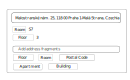
\includegraphics[width=\textwidth]{../img/address-mock}
	\caption{Mock of interactive address form}
	\label{fig:spec:addressmock}
\end{figure}

The address form needs to cover many specific scenarios. For example, users should also be able to specify addresses that can't be found by auto-complete functionality, even if such addresses can't be further separated into smaller fragments and queried by other applications. We will describe such specific requirements by the following list of use cases.

\begin{enumerate}[label=\color{usecasecolor}\textbf{U{\arabic*}}]
    \item \label{app:uc:event1} Specifying address with no auto-complete result
        \begin{enumerate}
            \item A user opens form to create a new event and set address value to auto-complete field
            \item Address auto-complete search provides no suggestions for specified value or auto-complete suggestion is not suitable to user
            \item User creates the event with initial address value selected
            \item Application stores provided address value as an generic address value described by single string
        \end{enumerate}
\end{enumerate}


Next to the data that can be structured, a user should be able to write any other information in a block of unstructured text. File attachments are an additional feature that would increase calendar usability. The calendar application should allow storing arbitrary attachments such as pictures, documents, or recordings.

\begin{enumerate}[label=\color{reqcolor}\textbf{R{\arabic*}}, resume]
    \item \label{app:req:events3} In calendar events, users can define the following unstructured data
        \begin{itemize}
            \item Optional description text
            \item Optional file attachments
        \end{itemize}
\end{enumerate}



\subsubsection*{Event Groups}

As calendar users utilize a calendar for many activities such as work meetings, university lectures, or their free time events, users should be able to differentiate between each specific type of activity visually. The present-day calendar applications introduced in section \ref{chap01:presentdaycals} also support such event grouping. Therefore, users should be able to categorize each event into a collection we call an \textit{event group}. Users can create an arbitrary number of event groups, each differentiable by group name and color. For example, figure \ref{fig:spec:eventgroups} shows a calendar with two event groups for work and school events.

\begin{figure}[!htb]
	\centering
	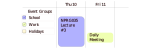
\includegraphics[width=\textwidth]{../img/event-groups}
	\caption{Example of two \textit{event groups} displayed in calendar}
	\label{fig:spec:eventgroups}
\end{figure}

To make application operations and user experience across the application more consistent, we define a rule that each event must belong to some group. If a user does not assign an event to some specific group, the application assigns the event to the default group. In addition, users can move each event group from one event group to another. In event group deletion, the calendar also removes all defined in the group.

\begin{enumerate}[label=\color{reqcolor}\textbf{R{\arabic*}}, resume]
    \item \label{app:req:groups1} Users can assign events into event groups.
        \begin{itemize}
            \item Users can create and remove own event groups.
            \item Application assigns a new calendar event to the \textit{default} event group if no user defined group is selected.
            \item Calendar events can be assigned from one calendar group to another.
        \end{itemize}
\end{enumerate}

\subsubsection*{Reccuring Events}



\begin{enumerate}[label=\color{reqcolor}\textbf{R{\arabic*}}, resume]
    \item \label{app:req:events4} User can define \textit{reccuring events}.
        \begin{itemize}
            \item Multiple future occurences of single reccuring event can be modified in single event update.
        \end{itemize}
\end{enumerate}

\subsubsection*{All-Day Events}

\subsection*{Calendar Views}
The application should support displaying calendar events in different calendar views, such as a view of calendar events in a single day, week or month. Views in different timespans increase the application's usability by hiding non-important events or providing a valuable overview of future events.
In the following subsection, we will introduce functional and non-functional requirements that each calendar view should support.

\begin{enumerate}[label=\color{reqcolor}\textbf{R{\arabic*}}, resume]
    \item \label{app:req:views0} Users should be able to display calendar events in a view displaying events of single day, week or month.
\end{enumerate}

\subsubsection*{Shared Functionality of Calendar Views}
In this subsection, we define a set of features that each calendar view should offer in the application. Defining such features increases the application's usability by defining expectable behavior shared in each calendar view.
As we want to make the calendar application interactive, users should be able to modify calendar events displayed in a calendar view by simply moving the visualization of the event from one timeslot to another. By modifying an event in a calendar view, users can set a different start time for an event or change the duration of an event, as shown in figure [X], where the user \textit{drag and drops} an event to a different location, changing start of the event.

\begin{enumerate}[label=\color{reqcolor}\textbf{R{\arabic*}}, resume]
    \item \label{app:req:views1} Users should be able to interactively modify start and duration of events displayed in calendar views.
    \item \label{app:req:views2} Users can create multiple instances of calendars view to display different calendar groups.
\end{enumerate}

\subsection*{Sharing}

One of the more advanced features of our application would be sharing calendar events with other application users. Users should be able to specify who can see and modify their events. The application should store user data only in SOLID Pod and follow other SOLID principles defined in the goal []. Therefore, Web Access Control, introduced in section [], will be used to implement calendar sharing features.

\begin{enumerate}[label=\color{reqcolor}\textbf{R{\arabic*}}, resume]
    \item \label{app:req:sharing1} User can create publicly shared calendar group that is readonly
    \item \label{app:req:sharing2} User can share calendar group only to group of users    
        \begin{itemize}
            \item Calendar group is privately shared and readonly
            \item Calendar group is privately shared and modifyable by each user with access
        \end{itemize}
    \item \label{app:req:sharing3} Users can create copy of other calendar groups that are shared with them
    \item \label{app:req:sharing4} Owner of calendar event can add participants to event
        \begin{itemize}
            \item Participants with access to the event can modify participation status
        \end{itemize}
\end{enumerate}

